\section{Model predictive control}\label{se:model_predictive_control}
In this section, the design of the controller is elaborated. First the control problem the design of the Model predictive controller (MPC). 

The simulation covered in chapter \ref{ch:simulation} is to be controlled with respect to the problems elaborated in section \ref{sec:problem_statement} and stated here. 
\begin{enumerate}
\item Flow variations due to large industries and natural phenomenons
\item Concentration variations due to large industries and natural phenomenons
\begin{enumerate}
	\item Chloride variations
	\item Phosphor variations
	\item Nitrogen variations
	\item Organic matter variations
\end{enumerate}
\end{enumerate}

From the problem statement, it is stated that flow and concentration variations must be kept to a minimum without causing any overflow in the sewer. To achieve this, tanks are used, these are placed in the sewer network to find locations where they are able to hold back disturbance that will otherwise cause flow and concentration variations into the WWTP. However, the output of these tanks must be controlled in a way where overflow in the tank is prohibited. Therefore the controller must control the output of these tanks in an optimal manner to keep the input variations to the WWTP at a minimum and still be controlled according to some constraints.

To obtain such an optimal behavior MPC is chosen as stated in section \ref{sec:problem_statement}. MPC solves a optimizations problem at each time instant, k, where the main point is to compute a control vector, u that is feed to the system. 

%is an advanced control method which depends on a dynamic model of the system. Where the model, constraints and a cost function is used to generate the most optimal sequence of control inputs to the system, thus obtaining a desired process behavior. However, only the first control input is used in the current timeslot. Hereafter, in the next timeslot, the MPC algorithm is recalculated to find the must optimal input signal for this timeslot and so on. In addition, MPC also take future disturbance into account thereby predicting an output sequence that is optimal including the disturbance. 
An MPC algorithm consists of:
\\ 
\textbf{Cost function} or control objective,$\CMcal{J}$, is an algorithm measuring e.g. the difference between future outputs and a reference while at the same time instant recognizing that any control action is costly for the system. Therefore the price is measured in the cost function over the prediction horizon, $H_p$. This function is therefore minimized with the respect to the future control vector to keep the cost minimized. Furthermore, only the first control input from the vector is used in each time instant thus this optimization is process is calculated at each time step where a new control input is calculated \cite{mpc_control_lecture_notes}.

\textbf{Constraints} is unique advantages of MPC. Constraints can be applied to the process variables e.g. constraints can be set on the states of the system not allowing them to go below a certain value or above. Constraints are usually written as inequality constraint $Ax\leq b$ where the constraint a subject to the optimization problem \cite{mpc_control_lecture_notes}.   

\textbf{Prediction model} for the MPC to be able to predict future system behavior it needs a model to predict from. The model describes the input output behavior of the system. The model will mainly be used to predict the output of the system over the prediction horizon \cite{mpc_control_lecture_notes}.  

% In figure \ref{fig:mpc_diagram} an illustration of a MPC controller is shown.
% \begin{figure}[H]
% 	\centering
% 	\includegraphics[width=0.60\textwidth]{report/control/pictures/mpc_diagram}
% 	\caption{Diagram of an MPC controller}
% 	\label{fig:mpc_diagram}
% \end{figure}



%The main advantage of MPC  Furthermore, MPC can be used with constraints to calculate the most optimal control output at the given timeslot and taking disturbance into the account. 
% In figure \ref{fig:control_of_sewer} it is shown that the MPC controller is setting the input to the pump.

% \begin{figure}[H]
% \centering
% \includegraphics[width=0.8\textwidth]{report/control/pictures/control_of_sewer.jpg}
% \caption{Block diagram of the system.}
% \label{fig:control_of_sewer}
% \end{figure}\fxnote{Der skal staa pumpe i stedet for tank}

% Where the iteration the in the MPC block can be described with the following items. 
% \begin{enumerate}
%        	\item Measurement is taken on the output if possible or it is taken directly from the states. If a state measurement is not available the state is estimated.
%        	\item Calculates a optimal set of predicted values over the prediction horizon according to a cost function and the constraints.
%        	\item The first element of the calculated control sequence is used as the control input.
%        	\item Repeat from 1.
% \end{enumerate}       

For MPC to optimize the system a cost function must be written to penalize variations of the flow output $Q(k+i|k)$ and the concentration output $C(k+i|k)$. Where k defines the prediction time and i is a value going from 1 to $H_p$. The cost function for flow and concentration is:

\begin{equation}
\begin{aligned}
	 \CMcal{J} &= \sum_{i=1}^{H_p-1} || Q(k+i|k)C_1(k+i|k)-Q(k+i-1|k)C_1(k+i-1|k)||_{\CMcal{Q}(i)}^2 \\&+\sum_{i=1}^{H_p-1} || Q(k+i|k)C_2(k+i|k)-Q(k+i-1|k)C_2(k+i-1|k)||_{\CMcal{Q}(i)}^2 \\&+\sum_{i=1}^{H_p-1} || Q(k+i|k)C_3(k+i|k)-Q(k+i-1|k)C_3(k+i-1|k)||_{\CMcal{Q}(i)}^2\\&+\sum_{i=1}^{H_p-1} || Q(k+i|k)C_4(k+i|k)-Q(k+i-1|k)C_4(k+i-1|k)||_{\CMcal{Q}(i)}^2 \\& +\sum_{i=1}^{H_p-1} || Q(k+i|k)-Q(k+i-1|k)||_{\CMcal{Q}(i)}^2
\end{aligned}	
\end{equation}\fxnote{skal skrives så alle 4 koncentrationer er med, samt en for flow og et eller andet sted afgrænsning for liggetid i tank}
Where $\CMcal{J}$ is the cost function that needs to be minimized, Q is the flow, C is the concentration and $\CMcal{Q}$ is a weighting parameter. The concentrations $C_1, C_2, C_3$ and $C_4$ are respectively chloride, phosphor nitrogen and organic matter levels in the wastewater.However, It has been chosen to only look at flow variation in the simulation and thereby excluding concentrations from the cost function and retention time in the tank\fxnote{enten skal vi fra vaelge os den noget før eller os skal vi have fundet på en cost function til liggetid}. This has been done to limit the control problem and ease the computation, to begin with. Thereby the cost function has been rewritten to: 

\begin{equation}\label{eq:cost_function_height}
	 \CMcal{J} = \sum_{i=1}^{H_p-1} || \hat{y}(k+i|k)-\hat{y}(k+i-1|k)||_{\CMcal{Q}(i)}^2
\end{equation}
\begin{equation}
	\begin{aligned}
	\text{s.t.} \hspace{5mm}  \hat{x}(k+i+1) &= A\hat{x}(k+i|k)+B\hat{u}(k+i|k)+B_dd(k+i|k) \\
						      \hat{y}(k+i)&= C\hat{x}(k+i|k) \\
						     \underline{x} \leq \hat{x} \leq \overline{x}
	\end{aligned}
\end{equation}
Where Q has been replaced with the output y as it can be measured directly from the state space system. The hat denotes a small signal value and not an estimate for y. y corresponds to the height of the wastewater in the channel, however, it is the same to minimize height difference as the flow because both describe the variation in the output of the sewer. Furthermore, the cost function is subject to constraints for the states. The states have a lower and upper constraint corresponding respectively to the bottom of the channel and the top of the channel, denoted respectively with $\underline{x}$ and $\overline{x}$. In order for the controller to minimize the variations in the output, it must be able to predict future events from knowing the current state. Therefore, by iterating the linear model up to the prediction horizon the controller is able to predict future states \cite{maciejowski2002predictive}. Thus by using the state equation recursively the state equation can be predicted up to the prediction horizon as shown in equation \ref{eq:iterating_state_equation}: 

\begin{equation}\label{eq:iterating_state_equation}
\begin{aligned}
	\hat{x}(k+1|k) &= A\hat{x}(k|k)+B\hat{u}(k|k) + B_dd(k|k)\\
	\hat{x}(k+2|k) &= A\hat{x}(k+1|k)+B\hat{u}(k+1|k)+ B_dd(k+1|k) \\
				   &= A^2\hat{x}(k|k)+AB\hat{u}(k|k)+AB_dd(k|k) + B\hat{u}(k+1|k) \\
				   &+ B_dd(k+1|k) \\
				   &\hspace{2mm}\vdots\\
   \hat{x}(k+H_p|k)&= A\hat{x}(k+H_p-1|k)+B\hat{u}(k+H_p-1|k)+B_dd(k+H_p-1|k)\\
   				   &= A^{H_p}\hat{x}(k|k)+A^{H_p-1}B\hat{u}(k|k)+A^{H_p-1}B_dd(k|k)+\cdots+\\
   				   &+B\hat{u}(k+H_p-1|k)+B_dd(k+H_p-1|k)
\end{aligned}
\end{equation}
Here the first equation $\hat{x}(k+1|k)$ is inserted into the second and this is iterated up to the prediction horizon. This can be setup as prediction vectors and matrices denoted by $\CMcal{X,A,B,U,B}_d$ and $\CMcal{D}$:


\begin{equation}\label{eq:lifted_state_equation}
\begin{aligned}
	  \underbrace{\begin{bmatrix}
	  \hat{x}(k+1|k) 	\\
	  \hat{x}(k+2|k) 	\\
	  \vdots 			\\
	  \hat{x}(k+H_p|k) 	\\
	   \end{bmatrix}}_{\CMcal{X}}
	 &=
	\underbrace{\begin{bmatrix}
		A \\
		A^2 \\
		\vdots \\
		A^{H_p} \\
	\end{bmatrix}}_{\CMcal{A}}
	\hat{x}(k|k) \\&+
	\underbrace{\begin{bmatrix}
		B 		 &0			 &\cdots	& 0		\\
		AB  	 &B  		 & \cdots& 0		\\
		\vdots 	 &\vdots	 & \ddots&\vdots	\\
		A^{H_p-1}B&A^{H_p-2}B&\cdots &B 
    \end{bmatrix}}_{\CMcal{B}}
    	\underbrace{\begin{bmatrix}
	\hat{u}(k|k)\\
	\hat{u}(k+1|k)\\
	\vdots\\
	\hat{u}(k+H_p-1|k)
	\end{bmatrix}}_{\CMcal{U}} \\ &+ 
    \underbrace{\begin{bmatrix}
    	B_d 	    &0	         &\cdots & 0		\\
		AB_d  	    &B_d  	     & \cdots& 0		\\
		\vdots 	    &\vdots	     & \ddots&\vdots	\\
		A^{H_p-1}B_d&A^{H_p-2}B_d&\cdots &B_d 
 %   	B & \cdots & 0 \\
 %    	AB+B & \cdots & 0 \\
 %    	\vdots & \ddots & \vdots \\
 %    	\sum_{i=0}^{H_u-1}A^i B & \cdots & B \\
 %    	\sum_{i=0}^{H_u}A^i B & \cdots & AB+B\\
 %    	\vdots & \vdots & \vdots \\
 %    	\sum_{i=0}^{H_p-1}A^i B & \cdots & \sum_{i=0}^{H_p-H_u}A^i B \\
	  \end{bmatrix}}_{\CMcal{B}_d} 
	\underbrace{\begin{bmatrix}
	\hat{d}(k|k)\\
	\hat{d}(k+1|k)\\
	\vdots\\
	\hat{d}(k+H_p-1|k)
	\end{bmatrix}}_{\CMcal{D}}
	\end{aligned}
\end{equation}

Where $\CMcal{X}$ is the predicted state vector for the entire prediction horizon. $\CMcal{A}$ is the state matrix up to the prediction horizon. $x(k|k)$ is the initial state and is used to predict the hole prediction horizon, $\CMcal{B}$ is the input matrix for the prediction horizon, $\CMcal{U}$ is the predicted input vector, which consists of all the predicted inputs from the current timestep until $(k+H_p-1)$. $\CMcal{B}_d$ is the disturbance matrix for the prediction horizon and $\CMcal{D}$ is the disturbance vector. 

This iteration process is also done for the output equation:

\begin{equation}\label{eq:lifted_output_equation}
	\CMcal{Y}(k)= 
	\begin{bmatrix}
	\hat{y}(k+1|k)\\
	\hat{y}(k+2|k)\\
	\vdots\\
	\hat{y}(k+H_p-1|k)
	\end{bmatrix}
	= 
	\underbrace{\begin{bmatrix}
	C 		& 0 	&\cdots	& 0\\
	0 		& C 	&\cdots & 0 \\
	\vdots	& \vdots&\ddots & 0\\
	0 		& 0		&0 		& C
	\end{bmatrix}}_{\CMcal{C}}
	  \begin{bmatrix}
	  \hat{x}(k+1|k) 	\\
	  \hat{x}(k+2|k) 	\\
	  \vdots 			\\
	  \hat{x}(k+H_p|k) 	\\
	   \end{bmatrix}
\end{equation}
Where $\CMcal{C}$ is a diagonal matrix with the output matrix C and $\CMcal{X}$ the predicted state vector. By inserting the predicted state equation \ref{eq:lifted_state_equation}, into the predicted output equation \ref{eq:lifted_output_equation} the following is achieved:

\begin{equation}\label{eq:output_eq_with_state_eq}
	\CMcal{Y}(k) =  \CMcal{C}\CMcal{A}x(k) +  \CMcal{C}\CMcal{B}\CMcal{U}(k) +\CMcal{C}\CMcal{B}_d\CMcal{D}(k)
\end{equation}   

By using the following notation on equation \ref{eq:output_eq_with_state_eq}:


\begin{equation}
 \psi = \CMcal{C}\CMcal{A}  \hspace{5mm} \gamma = \CMcal{C}\CMcal{B} \hspace{5mm}  \Theta = \CMcal{C}\CMcal{B}_{d}
\end{equation}

The predicted output equation can be rewritten as: 

\begin{equation}\label{eq:lifted_output_with_states_inserted}
	\CMcal{Y}(k) = \psi x(k) + \gamma \CMcal{U}(k) + \Theta \CMcal{D}(k)
\end{equation}

To be able to use the cost function, equation \ref{eq:cost_function_height}, it has to be rewritten so the predicted output equation can be used. This is done by replacing the output y with the predicted output $\CMcal{Y}$ thereby the following is obtained:

\begin{equation}
	\CMcal{J} = ||\CMcal{Y}(k)-\CMcal{Y}(k-1)||_{\CMcal{Q}(i)}^2
\end{equation}
Where the difference between $\CMcal{Y}(k)$ and $\CMcal{Y}(k-1)$ can be expressed as:

\begin{equation}
	\Delta \CMcal{Y}(k) =\CMcal{Y}(k)-\CMcal{Y}(k-1) 
\end{equation}

Thereby the following cost function is achieved:

\begin{equation}\label{eq:delta_cost_function}
	J = \Delta\CMcal{Y}(k)^T \cdot Q \cdot \Delta\CMcal{Y}(k)
\end{equation}

To be able to write the cost function as quadratic and linear terms of the predicted output $\Delta\CMcal{U}$, equation \ref{eq:lifted_output_with_states_inserted} is therefore inserted into equation \ref{eq:delta_cost_function} and thereby the following is obtained:

\begin{equation}\label{eq:cost_function_with_all_the_crap}
	\CMcal{J} = (\psi\Delta \hat{x}(k) + \gamma\Delta \CMcal{U}(k) + \Theta\Delta \CMcal{D}(k))^T\cdot Q \cdot (\psi\Delta \hat{x}(k) + \gamma\Delta \CMcal{U}(k) + \Theta\Delta \CMcal{D}(k))
\end{equation}

The term on the right hand side of equation \ref{eq:cost_function_with_all_the_crap} is equal to:

\begin{equation}\label{eq:cost_function_big_eq}
	\begin{aligned}
	&(\psi\Delta \hat{x}(k) + \gamma\Delta \CMcal{U}(k) + \Theta\Delta \CMcal{D}(k))^T\cdot Q \cdot (\psi\Delta \hat{x}(k) + \gamma\Delta \CMcal{U}(k) + \Theta\Delta \CMcal{D}(k)) = \\
	& \Delta \hat{x}(k)^T\psi ^T Q \psi \Delta \hat{x}(k) + \underbrace{\Delta \hat{x}(k)^T \psi ^T Q \gamma \Delta  \CMcal{U}(k) }_{Linear} +\Delta \hat{x}(k)^T \psi ^T Q \Theta \Delta \CMcal{D}(k) \\
	& \underbrace{\Delta \CMcal{U}(k)^T \gamma ^T Q \psi\Delta \hat{x}(k)}_{Linear} + \underbrace{\Delta \CMcal{U}(k)^T\gamma ^T Q \gamma\Delta \CMcal{U}(k)}_{Quadratic} +\underbrace{\Delta \CMcal{U}(k)^T \gamma ^T Q\Theta \Delta \CMcal{D}(k)}_{Linear} \\ 
	& \Delta \CMcal{D}(k)^T \Theta ^T Q  \psi \Delta \hat{x}(k)					+ \underbrace{\Delta \CMcal{D}(k)^T \Theta ^T Q \gamma  \Delta \CMcal{U}(k) }_{Linear}	+\Delta \CMcal{D}(k)^T \Theta ^T Q \Theta \Delta \CMcal{D}(k)
	\end{aligned}
\end{equation}

Here the quadratic and linear terms of $\Delta \CMcal{U}$ are denoted respectively, the remaining terms are the constants and these are not denoted in the equation, however, they will be referred to in the following equations as, c. The quadratic variables are collected in: 

\begin{equation}\label{eq:quadratic_h_matrix}
	\CMcal{H} = \gamma^T Q\gamma 
\end{equation}

And the linear variables are collected in:
\begin{equation}
	\begin{aligned}
	\CMcal{G} &= 2 \Delta \hat{x}(k)^T\psi^T Q \gamma+2 \Delta \CMcal{D}(k)^T\Theta^T Q \gamma 
	\end{aligned}
\end{equation}

Thereby inserting these expressions in equation \ref{eq:cost_function_big_eq} the final cost function is obtained:

\begin{equation}\label{eq:the_cost_function}
	\min_{\Delta \CMcal{U}(k)} \CMcal{J}(\Delta \CMcal{U}(k)) =\min_{\Delta \CMcal{U}(k)} \Delta \CMcal{U}(k)^T\CMcal{H}\Delta \CMcal{U}(k)+\CMcal{G}\Delta \CMcal{U}(k)+c
\end{equation}

\subsection{Constraints}\label{subse:constraints}

In order to apply the constraints, shown in equation \ref{eq:cost_function_height} for the states, to the optimization problem in equation \ref{eq:the_cost_function} the constraints must be reformulated so they are a constraint of the controller input $\Delta\CMcal{U}$, therefore it is required to reformulate the inequalities constraints. 

The constraints applied to the states are upper and lower bound to the channel and the tank. This will not allow the simulation to overfill the channel or the tank, or to have a negative height in either of the two. In the following equation the constraint for the states are shown:  


\begin{equation}
    x_{min} \leq \CMcal{X}(k) \leq x_{max}
\end{equation}

Where $x_{min}$ and $x_{max}$ are respectively lower and upper bound. As the constraint needs to be for small signal value and as the constraint is for full signal values the operating point needs to be subtracted from the lower and upper bounds thereby transforming the constraint into small signals:

\begin{equation}
    x_{min}- \bar{x} \leq \hat{\CMcal{X}}(k) \leq x_{max}-\bar{x}
\end{equation}

To reformulated the constraint the predicted state equation \ref{eq:lifted_state_equation} is inserted instead of the state vector.

\begin{equation}
     x_{min}- \bar{x} \leq \CMcal{A}\hat{x}(k)+\CMcal{B}\CMcal{U}(k)+\CMcal{BD}(k) \leq x_{max}-\bar{x}
 \end{equation} 

However, to make the constraint depend on $\Delta \CMcal{U}$ the difference between the current time step and the previous time step, $\CMcal{U}(k+n-1) = wu(k-1) +V\Delta \CMcal{U}(k+i-1) $, where w is a vector and V is a matrix on the form: 


This is inserted in the following equation: 

\begin{equation}
     x_{min}- \bar{x} \leq \CMcal{A}\hat{x}(k)+\CMcal{B}(\CMcal{U}(k-1)+\sum_{i=1}^n \Delta\CMcal{U}(k+i-1))+\CMcal{B}\CMcal{D}(k) \leq x_{max}-\bar{x}
 \end{equation} 


 Now the constraint is set up as a constraint on the input signal. In addition, the constraint has to be setup as equality constraints, therefore, it is divided into two constraints: 

 \begin{equation}
         \underbrace{\CMcal{B}\sum_{i=1}^n}_{\Lambda} \Delta\CMcal{U}(k+i-1)\leq \underbrace{x_{max}- \bar{x}-\CMcal{A}x(k)-\CMcal{B}\CMcal{U}(k-1)-\CMcal{B}\CMcal{D}(k)}_{\Gamma_1}
 \end{equation}  

 \begin{equation}
    -\underbrace{\CMcal{B}\sum_{i=1}^n}_{\Lambda} \Delta\CMcal{U}(k+i-1) \leq \underbrace{-x_{min}+\bar{x}+\CMcal{A}x(k)+\CMcal{B}\CMcal{U}(k-1)+\CMcal{B}\CMcal{D}(k)}_{\Gamma_2}
 \end{equation}


Constraints are also applied on the controller output. The reason for these constraints is to not allow the controller to produce a higher output than what the pipe after the tank is able to transport. The constraint for the controller output is construct in the same way as for the states in the system. Below the constraint for the controller output is shown:  
 \begin{equation}
 	u_{min} \leq \CMcal{U}(k) \leq u_{max}
 \end{equation}

The constraint needs to be written for small signal values, and needs to depend on the $\Delta \CMcal{U}$:

 \begin{equation}
 		u_{min} -  \bar{u} \leq \hat{\CMcal{U}}(k-1)+\sum_{i=1}^n \Delta\hat{\CMcal{U}}(k+i-1)  \leq  u_{max} -  \bar{u}
 \end{equation}

The constraint is split up into lower and upper bound for the signal, the upper bound is:

 \begin{equation}
 \begin{aligned}
			 	\hat{\CMcal{U}}(k-1)+\sum_{i=1}^n \Delta\hat{\CMcal{U}}(k+i-1)  &\leq  u_{max} -  \bar{u} \\
				\sum_{i=1}^n \Delta\hat{\CMcal{U}}(k+i-1)  &\leq  \underbrace{u_{max} -  \bar{u} - \hat{\CMcal{U}}(k-1)}_{\Gamma_3} \\
 \end{aligned}
 \end{equation}



And the lower bound:

 \begin{equation}
 \begin{aligned}
			 	u_{min} -  \bar{u} &\leq \hat{\CMcal{U}}(k-1)+\sum_{i=1}^n \Delta\hat{\CMcal{U}}(k+i-1) \\
-\sum_{i=1}^n \Delta\hat{\CMcal{U}}(k+i-1) &\leq \underbrace{\hat{\CMcal{U}}(k-1)-u_{min}+\bar{u}}_{\Gamma_4}
 \end{aligned}
 \end{equation}

The constraints can be setup on the standard inequality constraint form and thereby be included in the algorithm for the MPC implementation.

 \begin{equation}
        \begin{bmatrix}
           \Lambda\\
           -\Lambda\\
           \sum_{i=1}^n \\
           -\sum_{i=1}^n
           \end{bmatrix}
           \Delta\CMcal{U}
           \leq 
           \begin{bmatrix}
         \Gamma_{1.max}\\
         \Gamma_{2.min}\\
         \Gamma_{3.max}\\
         \Gamma_{4.min}

           \end{bmatrix}
 \end{equation}\label{eq:constriants_eq}

 In the following section the implementation of the cost function and constraints, shown in this section, in MATLAB will be elaborated

\subsection{Implementation of MPC}\label{subse:implementation_mpc}
In this section the implementation of MPC in MATLAB will be elaborated. 

The cost function in equation \ref{eq:the_cost_function} is a quadratic problem. In order to solve this minimization problem and find a global minimum quadratic programming (QP) is used. In MATLAB there well develop solvers for QP problems, in this project the quadprog function has been chosen. Quadprog solves the minimization problem subject to constraints to the specified convex cost function. The model used for the predictive model is the one covered in section \ref{se:linearization}. Furthermore, the constraints for the cost explained in the previous section will also be included. 

In figure \ref{fig:mpc_diagram} an illustration of a MPC controller is shown.
\begin{figure}[H]
	\centering
	\includegraphics[width=0.60\textwidth]{report/control/pictures/mpc_diagram}
	\caption{Diagram of an MPC controller}
	\label{fig:mpc_diagram}
\end{figure}

Here it is illustrated that the model, constraint and cost function will be used in the optimizer to generate an control output, that will be used in the process, which in this case is the nonlinear model. The output y(k+1) is the output height at the end of the last pipe in the sewer network. At each time step the current value of the output is feedback to the MPC controller. Here the MPC will at each iteration calculate up to $H_p$ control inputs, as it calculates for future disturbances, however, only the first element of this u vector will be used to control the process. Thereafter a new measurement will be taken and a new controller output will be calculated and this will iterate for the entire simulation.

In determining the length of the prediction horizon several considerations were taken into account. As illustration in section \ref{sec:WWTP_challenges} in figure \ref{fig:input_to_wwtp} a daily flow from the households is shown. Here the flow is illustrated for working days and in the weekend. Thereby by knowing the flow pattern for households the MPC would be able to include this knowledge in the prediction model. Thus ideal prediction horizon would be 24 hours, as it would be able to see the disturbance across a whole day. However, as the households are not the only disturbance in this setup this is not entirely true. Because the disturbance coming from the larger industry e.g. the bottling plant and the brewery are stochastic in a way, where it is unknown when the wastewater from the plants is coming and the periodicity between the outlets are unknown. Furthermore, the amount of wastewater coming from the plants are also different from time to time. Therefore, it would not be preferable to place the tank next to the industry as it would not be able to predict the disturbance. Thus the tank needs to be placed in a distance away from the industry, where it would be able to use the disturbance in the prediction model by knowing the disturbance coming from the industry by having a measurement of it. The time it takes the wastewater to leave the industry and to arrive at the tank would then decide the length of the prediction horizon. However, in the implementation of the MPC, it was discovered that the prediction horizon was restricted. Because when it was set to high, above 20, the quadratic $\CMcal{H}$ matrix, equation \ref{eq:quadratic_h_matrix}, was not semi-positive definite, as in the eigenvalues of it was negative, hence the quadratic problem was not convex. The reason for this problem is, that in the linearized model, some of the elements in matrices are very small and therefore, when the system is predicted, as shown in equation \ref{eq:lifted_state_equation}, the elements would be even smaller, thus causing the $\CMcal{H}$ matrix to have an extremely small negative eigenvalue. Therefore, several tests were conducted to find a prediction horizon that did not result in a negative eigenvalue. It was found that a prediction horizon of 20, thereby, the lowest eigenvalue of $\CMcal{H}$ was zero. However, this restricts the length of the pipe after the tank, because if the pipe is too long the MPC will not be able to predict all the way down to the output of it. Therefore, in the simulation of the MPC controller, this must be kept in mind.   

\subsection*{Results}
In the subsection the results obtained from the testing of the MPC controller will be covered. Two simulation will conducted, one where the constraints are neglected and therefore minimized without any restriction and another simulation where the constraints included. 

The pipe and tank setup for the simulation includes two pipes and one tank, where the tank is placed in the middle of the pipes. The specification for both pipes and the tank can be seen in tabular \ref{tab:pipe_data_for_mpc_test} and \ref{tab:tank_data_for_mpc_test} respectively.

\begin{table}[H]
\centering
\begin{tabular}{|c|c|c|c|c|c|c|c|}
\hline
\textbf{Pipe number} & \textbf{Length} [m] & \textbf{Sections} & \textbf{Dx} [m] & \textbf{Ib} & \textbf{d} [m] & \textbf{$\theta$} & \textbf{Qf $[m^3/s]$} \\ \hline
1&100             & 5                 & 20          & 0,003       & 0,9        & 0,65              & 0,97        \\ \hline
2&100             & 5                 & 20          & 0,003       & 0,9        & 0,65              & 0,97        \\ \hline
\end{tabular}
\caption{The pipe specification for the test.}
\label{tab:pipe_data_for_mpc_test}
\end{table}
\begin{table}[H]
\centering
\begin{tabular}{|c|c|}
\hline
\textbf{Size $[m^3]$}        & 90   \\ \hline
\textbf{Height $[m]$}      & 10   \\ \hline
\textbf{Area $[m^2]$}        & 9    \\ \hline
\textbf{Q\_out\_max} $[m^3/s]$& 0,97 \\ \hline
\end{tabular}
\caption{Tank specification for the test.}
\label{tab:tank_data_for_mpc_test}
\end{table}

In the first simulation the MPC controller is minimizing the output variations of the tank without any constraints included. The input signal in the first pipe is shown in figure \ref{fig:input_to_pipe_mpc_test}. 
\begin{figure}[H]
 \centering
 % This file was created by matlab2tikz.
%
%The latest updates can be retrieved from
%  http://www.mathworks.com/matlabcentral/fileexchange/22022-matlab2tikz-matlab2tikz
%where you can also make suggestions and rate matlab2tikz.
%
\definecolor{mycolor1}{rgb}{0.00000,0.44700,0.74100}%
%
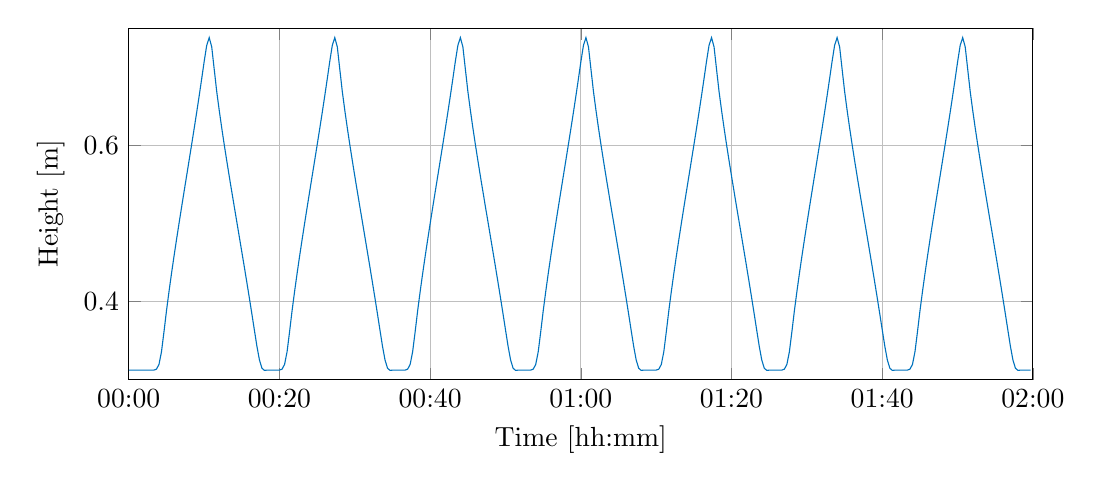
\begin{tikzpicture}

\begin{axis}[%
width=4.521in,
height=1.7566in,
at={(0.758in,0.481in)},
scale only axis,
xmin=0,
xmax=7200,
xtick={0,1200,2400,3600,4800,6000,7200},
xticklabels={{00:00},{00:20},{00:40},{01:00},{01:20},{01:40},{02:00},{},{}},
xlabel={Time [hh:mm]},
xmajorgrids,
ymin=0.3,
ymax=0.75,
ylabel={Height [m]},
ymajorgrids,
axis background/.style={fill=white}
]
\addplot [color=mycolor1,solid,forget plot]
  table[row sep=crcr]{%
1	0.312023249317626\\
21	0.312023246837098\\
41	0.312023246936918\\
61	0.31202324716405\\
81	0.312023247183117\\
101	0.312023246894595\\
121	0.312023246804861\\
141	0.312023246826466\\
161	0.312023246825577\\
181	0.312023246825557\\
201	0.312121005770395\\
221	0.313303250174373\\
241	0.319307912081077\\
261	0.33560042184716\\
281	0.361307543036265\\
301	0.388322628144609\\
321	0.412901747556437\\
341	0.436092176122273\\
361	0.458221284324029\\
381	0.479572705047134\\
401	0.500354828562447\\
421	0.520734810671735\\
441	0.540853079164184\\
461	0.560839003631458\\
481	0.580823234318298\\
501	0.600927924799851\\
521	0.621271058657982\\
541	0.641981241110515\\
561	0.663205613163634\\
581	0.685098848667415\\
601	0.70748595804283\\
621	0.727933515013021\\
641	0.737968475376296\\
661	0.726122858711694\\
681	0.697297259175176\\
701	0.668736952602323\\
721	0.644580482279641\\
741	0.621930351212498\\
761	0.600519192064094\\
781	0.579928262349129\\
801	0.559912955290504\\
821	0.540288675870878\\
841	0.520918920796392\\
861	0.50168824695521\\
881	0.482487723833863\\
901	0.46322159475537\\
921	0.443804175511088\\
941	0.424153152222034\\
961	0.404184540411282\\
981	0.383811358489671\\
1001	0.363040275945682\\
1021	0.342592073540271\\
1041	0.325074613474565\\
1061	0.314501198807809\\
1081	0.311713331931931\\
1101	0.312039913402904\\
1121	0.312022582385124\\
1141	0.312023269080089\\
1161	0.312023246137276\\
1181	0.312023246819224\\
1201	0.312121005770507\\
1221	0.313303250174375\\
1241	0.319307912081077\\
1261	0.33560042184716\\
1281	0.361307543036265\\
1301	0.388322628144609\\
1321	0.412901747556437\\
1341	0.436092176122273\\
1361	0.458221284324029\\
1381	0.479572705047134\\
1401	0.500354828562447\\
1421	0.520734810671735\\
1441	0.540853079164184\\
1461	0.560839003631458\\
1481	0.580823234318298\\
1501	0.600927924799851\\
1521	0.621271058657982\\
1541	0.641981241110515\\
1561	0.663205613163634\\
1581	0.685098848667415\\
1601	0.70748595804283\\
1621	0.727933515013021\\
1641	0.737968475376296\\
1661	0.726122858711694\\
1681	0.697297259175176\\
1701	0.668736952602323\\
1721	0.644580482279641\\
1741	0.621930351212498\\
1761	0.600519192064094\\
1781	0.579928262349129\\
1801	0.559912955290504\\
1821	0.540288675870878\\
1841	0.520918920796392\\
1861	0.50168824695521\\
1881	0.482487723833863\\
1901	0.46322159475537\\
1921	0.443804175511088\\
1941	0.424153152222034\\
1961	0.404184540411282\\
1981	0.383811358489671\\
2001	0.363040275945682\\
2021	0.342592073540271\\
2041	0.325074613474565\\
2061	0.314501198807809\\
2081	0.311713331931931\\
2101	0.312039913402904\\
2121	0.312022582385124\\
2141	0.312023269080089\\
2161	0.312023246137276\\
2181	0.312023246819224\\
2201	0.312121005770507\\
2221	0.313303250174375\\
2241	0.319307912081077\\
2261	0.33560042184716\\
2281	0.361307543036265\\
2301	0.388322628144609\\
2321	0.412901747556437\\
2341	0.436092176122273\\
2361	0.458221284324029\\
2381	0.479572705047134\\
2401	0.500354828562447\\
2421	0.520734810671735\\
2441	0.540853079164184\\
2461	0.560839003631458\\
2481	0.580823234318298\\
2501	0.600927924799851\\
2521	0.621271058657982\\
2541	0.641981241110515\\
2561	0.663205613163634\\
2581	0.685098848667415\\
2601	0.70748595804283\\
2621	0.727933515013021\\
2641	0.737968475376296\\
2661	0.726122858711694\\
2681	0.697297259175176\\
2701	0.668736952602323\\
2721	0.644580482279641\\
2741	0.621930351212498\\
2761	0.600519192064094\\
2781	0.579928262349129\\
2801	0.559912955290504\\
2821	0.540288675870878\\
2841	0.520918920796392\\
2861	0.50168824695521\\
2881	0.482487723833863\\
2901	0.46322159475537\\
2921	0.443804175511088\\
2941	0.424153152222034\\
2961	0.404184540411282\\
2981	0.383811358489671\\
3001	0.363040275945682\\
3021	0.342592073540271\\
3041	0.325074613474565\\
3061	0.314501198807809\\
3081	0.311713331931931\\
3101	0.312039913402904\\
3121	0.312022582385124\\
3141	0.312023269080089\\
3161	0.312023246137276\\
3181	0.312023246819224\\
3201	0.312121005770507\\
3221	0.313303250174375\\
3241	0.319307912081077\\
3261	0.33560042184716\\
3281	0.361307543036265\\
3301	0.388322628144609\\
3321	0.412901747556437\\
3341	0.436092176122273\\
3361	0.458221284324029\\
3381	0.479572705047134\\
3401	0.500354828562447\\
3421	0.520734810671735\\
3441	0.540853079164184\\
3461	0.560839003631458\\
3481	0.580823234318298\\
3501	0.600927924799851\\
3521	0.621271058657982\\
3541	0.641981241110515\\
3561	0.663205613163634\\
3581	0.685098848667415\\
3601	0.70748595804283\\
3621	0.727933515013021\\
3641	0.737968475376296\\
3661	0.726122858711694\\
3681	0.697297259175176\\
3701	0.668736952602323\\
3721	0.644580482279641\\
3741	0.621930351212498\\
3761	0.600519192064094\\
3781	0.579928262349129\\
3801	0.559912955290504\\
3821	0.540288675870878\\
3841	0.520918920796392\\
3861	0.50168824695521\\
3881	0.482487723833863\\
3901	0.46322159475537\\
3921	0.443804175511088\\
3941	0.424153152222034\\
3961	0.404184540411282\\
3981	0.383811358489671\\
4001	0.363040275945682\\
4021	0.342592073540271\\
4041	0.325074613474565\\
4061	0.314501198807809\\
4081	0.311713331931931\\
4101	0.312039913402904\\
4121	0.312022582385124\\
4141	0.312023269080089\\
4161	0.312023246137276\\
4181	0.312023246819224\\
4201	0.312121005770507\\
4221	0.313303250174375\\
4241	0.319307912081077\\
4261	0.33560042184716\\
4281	0.361307543036265\\
4301	0.388322628144609\\
4321	0.412901747556437\\
4341	0.436092176122273\\
4361	0.458221284324029\\
4381	0.479572705047134\\
4401	0.500354828562447\\
4421	0.520734810671735\\
4441	0.540853079164184\\
4461	0.560839003631458\\
4481	0.580823234318298\\
4501	0.600927924799851\\
4521	0.621271058657982\\
4541	0.641981241110515\\
4561	0.663205613163634\\
4581	0.685098848667415\\
4601	0.70748595804283\\
4621	0.727933515013021\\
4641	0.737968475376296\\
4661	0.726122858711694\\
4681	0.697297259175176\\
4701	0.668736952602323\\
4721	0.644580482279641\\
4741	0.621930351212498\\
4761	0.600519192064094\\
4781	0.579928262349129\\
4801	0.559912955290504\\
4821	0.540288675870878\\
4841	0.520918920796392\\
4861	0.50168824695521\\
4881	0.482487723833863\\
4901	0.46322159475537\\
4921	0.443804175511088\\
4941	0.424153152222034\\
4961	0.404184540411282\\
4981	0.383811358489671\\
5001	0.363040275945682\\
5021	0.342592073540271\\
5041	0.325074613474565\\
5061	0.314501198807809\\
5081	0.311713331931931\\
5101	0.312039913402904\\
5121	0.312022582385124\\
5141	0.312023269080089\\
5161	0.312023246137276\\
5181	0.312023246819224\\
5201	0.312121005770507\\
5221	0.313303250174375\\
5241	0.319307912081077\\
5261	0.33560042184716\\
5281	0.361307543036265\\
5301	0.388322628144609\\
5321	0.412901747556437\\
5341	0.436092176122273\\
5361	0.458221284324029\\
5381	0.479572705047134\\
5401	0.500354828562447\\
5421	0.520734810671735\\
5441	0.540853079164184\\
5461	0.560839003631458\\
5481	0.580823234318298\\
5501	0.600927924799851\\
5521	0.621271058657982\\
5541	0.641981241110515\\
5561	0.663205613163634\\
5581	0.685098848667415\\
5601	0.70748595804283\\
5621	0.727933515013021\\
5641	0.737968475376296\\
5661	0.726122858711694\\
5681	0.697297259175176\\
5701	0.668736952602323\\
5721	0.644580482279641\\
5741	0.621930351212498\\
5761	0.600519192064094\\
5781	0.579928262349129\\
5801	0.559912955290504\\
5821	0.540288675870878\\
5841	0.520918920796392\\
5861	0.50168824695521\\
5881	0.482487723833863\\
5901	0.46322159475537\\
5921	0.443804175511088\\
5941	0.424153152222034\\
5961	0.404184540411282\\
5981	0.383811358489671\\
6001	0.363040275945682\\
6021	0.342592073540271\\
6041	0.325074613474565\\
6061	0.314501198807809\\
6081	0.311713331931931\\
6101	0.312039913402904\\
6121	0.312022582385124\\
6141	0.312023269080089\\
6161	0.312023246137276\\
6181	0.312023246819224\\
6201	0.312121005770507\\
6221	0.313303250174375\\
6241	0.319307912081077\\
6261	0.33560042184716\\
6281	0.361307543036265\\
6301	0.388322628144609\\
6321	0.412901747556437\\
6341	0.436092176122273\\
6361	0.458221284324029\\
6381	0.479572705047134\\
6401	0.500354828562447\\
6421	0.520734810671735\\
6441	0.540853079164184\\
6461	0.560839003631458\\
6481	0.580823234318298\\
6501	0.600927924799851\\
6521	0.621271058657982\\
6541	0.641981241110515\\
6561	0.663205613163634\\
6581	0.685098848667415\\
6601	0.70748595804283\\
6621	0.727933515013021\\
6641	0.737968475376296\\
6661	0.726122858711694\\
6681	0.697297259175176\\
6701	0.668736952602323\\
6721	0.644580482279641\\
6741	0.621930351212498\\
6761	0.600519192064094\\
6781	0.579928262349129\\
6801	0.559912955290504\\
6821	0.540288675870878\\
6841	0.520918920796392\\
6861	0.50168824695521\\
6881	0.482487723833863\\
6901	0.46322159475537\\
6921	0.443804175511088\\
6941	0.424153152222034\\
6961	0.404184540411282\\
6981	0.383811358489671\\
7001	0.363040275945682\\
7021	0.342592073540271\\
7041	0.325074613474565\\
7061	0.314501198807809\\
7081	0.311713331931931\\
7101	0.312039913402904\\
7121	0.312022582385124\\
7141	0.312023269080089\\
7161	0.312023246137276\\
7181	0.312023246819224\\
};
\end{axis}
\end{tikzpicture}%
\caption{The input to the first pipe.}
\label{fig:input_to_pipe_mpc_test}
\end{figure}

Here there is a constant input of 0,2 $m^3/s$, which results in a height of 0,31 meters in the pipe. On top of the input a disturbance signal is added. This is done to see if the MPC is able to keep the flow variations out of the tank to a minimum. This signal is a upper triangular signal which goes from the constant input up to 0,9 $m^3/s$ which is equal to a height of 0,75 meters in the pipe. The time between each disturbance signal is 200 seconds and the period of the triangle signal is 100 seconds. This simulation conducted for two hours where $\Delta t$ is 20 seconds. In figure \ref{fig:MPC_test_output_first_test} the output of the the last pipe is shown.  


\begin{figure}[H]
 \centering
 % This file was created by matlab2tikz.
%
%The latest updates can be retrieved from
%  http://www.mathworks.com/matlabcentral/fileexchange/22022-matlab2tikz-matlab2tikz
%where you can also make suggestions and rate matlab2tikz.
%
\definecolor{mycolor1}{rgb}{0.00000,0.44700,0.74100}%
%
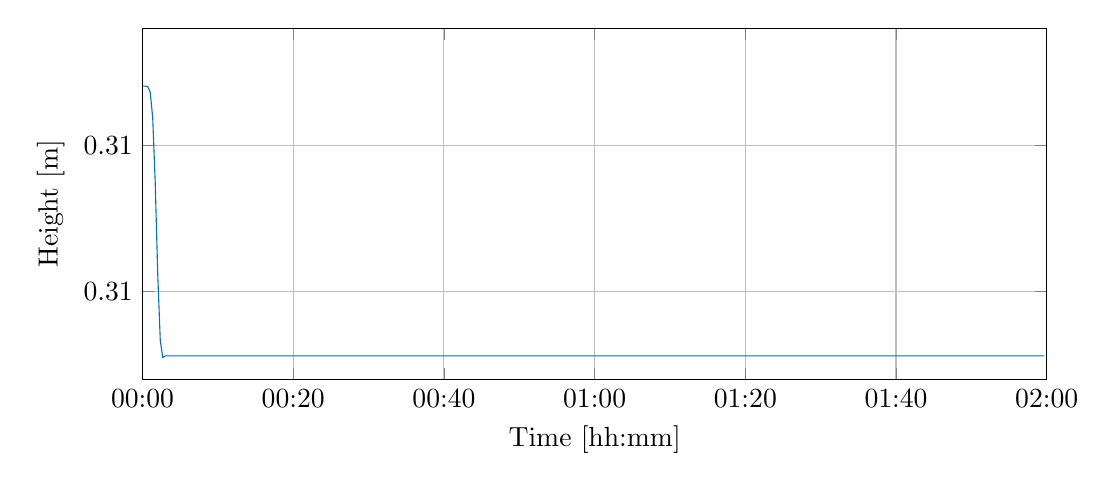
\begin{tikzpicture}

\begin{axis}[%
width=4.521in,
height=1.7566in,
at={(0.758in,0.481in)},
scale only axis,
xmin=0,
xmax=7200,
xtick={0,1200,2400,3600,4800,6000,7200},
xticklabels={{00:00},{00:20},{00:40},{01:00},{01:20},{01:40},{02:00},{},{}},
xlabel={Time [hh:mm]},
xmajorgrids,
ymin=0.302,
ymax=0.314,
ylabel={Height [m]},
ymajorgrids,
axis background/.style={fill=white}
]
\addplot [color=mycolor1,solid,forget plot]
  table[row sep=crcr]{%
1	0.312023251728134\\
21	0.312023249248491\\
41	0.312007329576048\\
61	0.311822355594219\\
81	0.310938012057319\\
101	0.308710026090253\\
121	0.305594844450276\\
141	0.303344739104071\\
161	0.302753859420006\\
181	0.302809429127008\\
201	0.30280716177161\\
221	0.302807232518793\\
241	0.302807230514799\\
261	0.302807230566105\\
281	0.30280723056466\\
301	0.302807230564718\\
321	0.302807230564717\\
341	0.302807230564717\\
361	0.302807230564717\\
381	0.302807230564717\\
401	0.302807230564717\\
421	0.302807230564717\\
441	0.302807230564717\\
461	0.302807230564717\\
481	0.302807230564717\\
501	0.302807230564717\\
521	0.302807230564717\\
541	0.302807230564717\\
561	0.302807230564717\\
581	0.302807230564717\\
601	0.302807230564717\\
621	0.302807230564717\\
641	0.302807230564717\\
661	0.302807230564717\\
681	0.302807230564717\\
701	0.302807230564717\\
721	0.302807230564717\\
741	0.302807230564717\\
761	0.302807230564717\\
781	0.302807230564717\\
801	0.302807230564717\\
821	0.302807230564717\\
841	0.302807230564717\\
861	0.302807230564717\\
881	0.302807230564717\\
901	0.302807230564717\\
921	0.302807230564717\\
941	0.302807230564717\\
961	0.302807230564717\\
981	0.302807230564717\\
1001	0.302807230564717\\
1021	0.302807230564717\\
1041	0.302807230564717\\
1061	0.302807230564717\\
1081	0.302807230564717\\
1101	0.302807230564717\\
1121	0.302807230564717\\
1141	0.302807230564717\\
1161	0.302807230564717\\
1181	0.302807230564717\\
1201	0.302807230564717\\
1221	0.302807230564717\\
1241	0.302807230564717\\
1261	0.302807230564717\\
1281	0.302807230564717\\
1301	0.302807230564717\\
1321	0.302807230564717\\
1341	0.302807230564717\\
1361	0.302807230564717\\
1381	0.302807230564717\\
1401	0.302807230564717\\
1421	0.302807230564717\\
1441	0.302807230564717\\
1461	0.302807230564717\\
1481	0.302807230564717\\
1501	0.302807230564717\\
1521	0.302807230564717\\
1541	0.302807230564717\\
1561	0.302807230564717\\
1581	0.302807230564717\\
1601	0.302807230564717\\
1621	0.302807230564717\\
1641	0.302807230564717\\
1661	0.302807230564717\\
1681	0.302807230564717\\
1701	0.302807230564717\\
1721	0.302807230564717\\
1741	0.302807230564717\\
1761	0.302807230564717\\
1781	0.302807230564717\\
1801	0.302807230564717\\
1821	0.302807230564717\\
1841	0.302807230564717\\
1861	0.302807230564717\\
1881	0.302807230564717\\
1901	0.302807230564717\\
1921	0.302807230564717\\
1941	0.302807230564717\\
1961	0.302807230564717\\
1981	0.302807230564717\\
2001	0.302807230564717\\
2021	0.302807230564717\\
2041	0.302807230564717\\
2061	0.302807230564717\\
2081	0.302807230564717\\
2101	0.302807230564717\\
2121	0.302807230564717\\
2141	0.302807230564717\\
2161	0.302807230564717\\
2181	0.302807230564717\\
2201	0.302807230564717\\
2221	0.302807230564717\\
2241	0.302807230564717\\
2261	0.302807230564717\\
2281	0.302807230564717\\
2301	0.302807230564717\\
2321	0.302807230564717\\
2341	0.302807230564717\\
2361	0.302807230564717\\
2381	0.302807230564717\\
2401	0.302807230564717\\
2421	0.302807230564717\\
2441	0.302807230564717\\
2461	0.302807230564717\\
2481	0.302807230564717\\
2501	0.302807230564717\\
2521	0.302807230564717\\
2541	0.302807230564717\\
2561	0.302807230564717\\
2581	0.302807230564717\\
2601	0.302807230564717\\
2621	0.302807230564717\\
2641	0.302807230564717\\
2661	0.302807230564717\\
2681	0.302807230564717\\
2701	0.302807230564717\\
2721	0.302807230564717\\
2741	0.302807230564717\\
2761	0.302807230564717\\
2781	0.302807230564717\\
2801	0.302807230564717\\
2821	0.302807230564717\\
2841	0.302807230564717\\
2861	0.302807230564717\\
2881	0.302807230564717\\
2901	0.302807230564717\\
2921	0.302807230564717\\
2941	0.302807230564717\\
2961	0.302807230564717\\
2981	0.302807230564717\\
3001	0.302807230564717\\
3021	0.302807230564717\\
3041	0.302807230564717\\
3061	0.302807230564717\\
3081	0.302807230564717\\
3101	0.302807230564717\\
3121	0.302807230564717\\
3141	0.302807230564717\\
3161	0.302807230564717\\
3181	0.302807230564717\\
3201	0.302807230564717\\
3221	0.302807230564717\\
3241	0.302807230564717\\
3261	0.302807230564717\\
3281	0.302807230564717\\
3301	0.302807230564717\\
3321	0.302807230564717\\
3341	0.302807230564717\\
3361	0.302807230564717\\
3381	0.302807230564717\\
3401	0.302807230564717\\
3421	0.302807230564717\\
3441	0.302807230564717\\
3461	0.302807230564717\\
3481	0.302807230564717\\
3501	0.302807230564717\\
3521	0.302807230564717\\
3541	0.302807230564717\\
3561	0.302807230564717\\
3581	0.302807230564717\\
3601	0.302807230564717\\
3621	0.302807230564717\\
3641	0.302807230564717\\
3661	0.302807230564717\\
3681	0.302807230564717\\
3701	0.302807230564717\\
3721	0.302807230564717\\
3741	0.302807230564717\\
3761	0.302807230564717\\
3781	0.302807230564717\\
3801	0.302807230564717\\
3821	0.302807230564717\\
3841	0.302807230564717\\
3861	0.302807230564717\\
3881	0.302807230564717\\
3901	0.302807230564717\\
3921	0.302807230564717\\
3941	0.302807230564717\\
3961	0.302807230564717\\
3981	0.302807230564717\\
4001	0.302807230564717\\
4021	0.302807230564717\\
4041	0.302807230564717\\
4061	0.302807230564717\\
4081	0.302807230564717\\
4101	0.302807230564717\\
4121	0.302807230564717\\
4141	0.302807230564717\\
4161	0.302807230564717\\
4181	0.302807230564717\\
4201	0.302807230564717\\
4221	0.302807230564717\\
4241	0.302807230564717\\
4261	0.302807230564717\\
4281	0.302807230564717\\
4301	0.302807230564717\\
4321	0.302807230564717\\
4341	0.302807230564717\\
4361	0.302807230564717\\
4381	0.302807230564717\\
4401	0.302807230564717\\
4421	0.302807230564717\\
4441	0.302807230564717\\
4461	0.302807230564717\\
4481	0.302807230564717\\
4501	0.302807230564717\\
4521	0.302807230564717\\
4541	0.302807230564717\\
4561	0.302807230564717\\
4581	0.302807230564717\\
4601	0.302807230564717\\
4621	0.302807230564717\\
4641	0.302807230564717\\
4661	0.302807230564717\\
4681	0.302807230564717\\
4701	0.302807230564717\\
4721	0.302807230564717\\
4741	0.302807230564717\\
4761	0.302807230564717\\
4781	0.302807230564717\\
4801	0.302807230564717\\
4821	0.302807230564717\\
4841	0.302807230564717\\
4861	0.302807230564717\\
4881	0.302807230564717\\
4901	0.302807230564717\\
4921	0.302807230564717\\
4941	0.302807230564717\\
4961	0.302807230564717\\
4981	0.302807230564717\\
5001	0.302807230564717\\
5021	0.302807230564717\\
5041	0.302807230564717\\
5061	0.302807230564717\\
5081	0.302807230564717\\
5101	0.302807230564717\\
5121	0.302807230564717\\
5141	0.302807230564717\\
5161	0.302807230564717\\
5181	0.302807230564717\\
5201	0.302807230564717\\
5221	0.302807230564717\\
5241	0.302807230564717\\
5261	0.302807230564717\\
5281	0.302807230564717\\
5301	0.302807230564717\\
5321	0.302807230564717\\
5341	0.302807230564717\\
5361	0.302807230564717\\
5381	0.302807230564717\\
5401	0.302807230564717\\
5421	0.302807230564717\\
5441	0.302807230564717\\
5461	0.302807230564717\\
5481	0.302807230564717\\
5501	0.302807230564717\\
5521	0.302807230564717\\
5541	0.302807230564717\\
5561	0.302807230564717\\
5581	0.302807230564717\\
5601	0.302807230564717\\
5621	0.302807230564717\\
5641	0.302807230564717\\
5661	0.302807230564717\\
5681	0.302807230564717\\
5701	0.302807230564717\\
5721	0.302807230564717\\
5741	0.302807230564717\\
5761	0.302807230564717\\
5781	0.302807230564717\\
5801	0.302807230564717\\
5821	0.302807230564717\\
5841	0.302807230564717\\
5861	0.302807230564717\\
5881	0.302807230564717\\
5901	0.302807230564717\\
5921	0.302807230564717\\
5941	0.302807230564717\\
5961	0.302807230564717\\
5981	0.302807230564717\\
6001	0.302807230564717\\
6021	0.302807230564717\\
6041	0.302807230564717\\
6061	0.302807230564717\\
6081	0.302807230564717\\
6101	0.302807230564717\\
6121	0.302807230564717\\
6141	0.302807230564717\\
6161	0.302807230564717\\
6181	0.302807230564717\\
6201	0.302807230564717\\
6221	0.302807230564717\\
6241	0.302807230564717\\
6261	0.302807230564717\\
6281	0.302807230564717\\
6301	0.302807230564717\\
6321	0.302807230564717\\
6341	0.302807230564717\\
6361	0.302807230564717\\
6381	0.302807230564717\\
6401	0.302807230564717\\
6421	0.302807230564717\\
6441	0.302807230564717\\
6461	0.302807230564717\\
6481	0.302807230564717\\
6501	0.302807230564717\\
6521	0.302807230564717\\
6541	0.302807230564717\\
6561	0.302807230564717\\
6581	0.302807230564717\\
6601	0.302807230564717\\
6621	0.302807230564717\\
6641	0.302807230564717\\
6661	0.302807230564717\\
6681	0.302807230564717\\
6701	0.302807230564717\\
6721	0.302807230564717\\
6741	0.302807230564717\\
6761	0.302807230564717\\
6781	0.302807230564717\\
6801	0.302807230564717\\
6821	0.302807230564717\\
6841	0.302807230564717\\
6861	0.302807230564717\\
6881	0.302807230564717\\
6901	0.302807230564717\\
6921	0.302807230564717\\
6941	0.302807230564717\\
6961	0.302807230564717\\
6981	0.302807230564717\\
7001	0.302807230564717\\
7021	0.302807230564717\\
7041	0.302807230564717\\
7061	0.302807230564717\\
7081	0.302807230564717\\
7101	0.302807230564717\\
7121	0.302807230564717\\
7141	0.302807230564717\\
7161	0.302807230564717\\
7181	0.302807230564717\\
};
\end{axis}
\end{tikzpicture}%
\caption{The output of the last pipe.}
\label{fig:MPC_test_output_first_test}
\end{figure}

Here it can be seen that the MPC controller is able to minimize the disturbance coming from the first pipe as the output is constant. At the beginning the height of the output is a bit higher, this is due to that the tank holds wastewater at the beginning of the simulation. After it is emptied the height falls down to a constant level. In figure \ref{fig:tank_height_first_test} the height in the tank can be seen.  

\begin{figure}[H]
 \centering
 % This file was created by matlab2tikz.
%
%The latest updates can be retrieved from
%  http://www.mathworks.com/matlabcentral/fileexchange/22022-matlab2tikz-matlab2tikz
%where you can also make suggestions and rate matlab2tikz.
%
\definecolor{mycolor1}{rgb}{0.00000,0.44700,0.74100}%
%
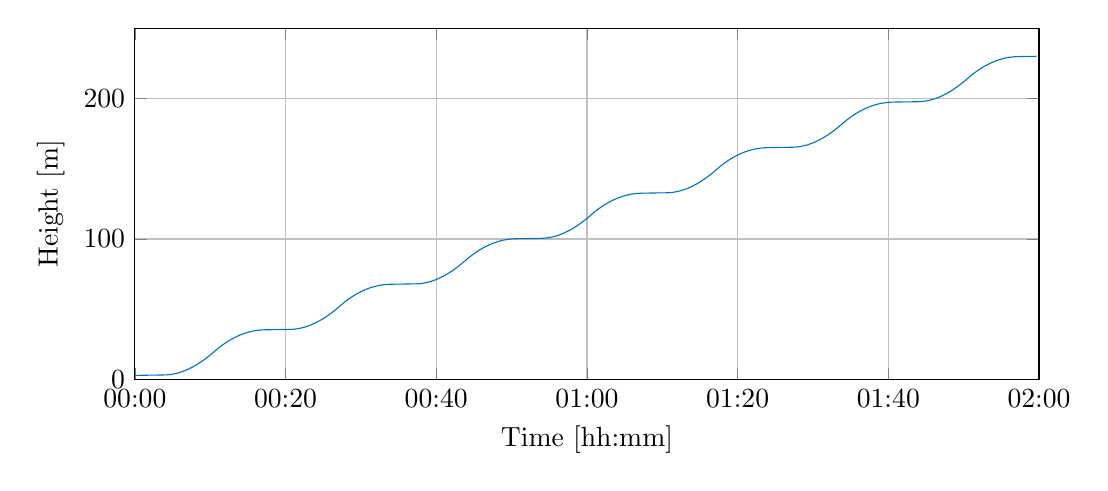
\begin{tikzpicture}

\begin{axis}[%
width=4.521in,
height=1.7566in,
at={(0.758in,0.481in)},
scale only axis,
xmin=0,
xmax=7200,
xtick={0,1200,2400,3600,4800,6000,7200},
xticklabels={{00:00},{00:20},{00:40},{01:00},{01:20},{01:40},{02:00},{},{}},
xlabel={Time [hh:mm]},
xmajorgrids,
ymin=0,
ymax=250,
ylabel={Height [m]},
ymajorgrids,
axis background/.style={fill=white}
]
\addplot [color=mycolor1,solid,forget plot]
  table[row sep=crcr]{%
1	3\\
21	2.99999999316026\\
41	3.01333332012207\\
61	3.03959998125893\\
81	3.06547864251583\\
101	3.0913689429355\\
121	3.11725889387259\\
141	3.14314885534856\\
161	3.16903881650788\\
181	3.19492877767658\\
201	3.22109726239619\\
221	3.25064049511399\\
241	3.29750672298085\\
261	3.39288632107958\\
281	3.56912437310451\\
301	3.83562039561864\\
321	4.1884579507952\\
341	4.62596199875373\\
361	5.14668512035647\\
381	5.7494827934806\\
401	6.43337998659827\\
421	7.19750182241436\\
441	8.04101866643031\\
461	8.96312223426952\\
481	9.96302380040749\\
501	11.039887872545\\
521	12.1927572414809\\
541	13.4205046227795\\
561	14.7217726784438\\
581	16.0948253034624\\
601	17.5363557398054\\
621	19.0355207754558\\
641	20.561105099706\\
661	22.0553687508651\\
681	23.4663940829603\\
701	24.7862125447617\\
721	26.0231507287676\\
741	27.1784456543558\\
761	28.2537615398048\\
781	29.250202800168\\
801	30.1686784502063\\
821	31.0099695548669\\
841	31.7748177980667\\
861	32.4639480818204\\
881	33.078059988109\\
901	33.6178651508038\\
921	34.0841268148811\\
941	34.4776849406166\\
961	34.7994733082725\\
981	35.0505432017909\\
1001	35.2324131711823\\
1021	35.3492728058711\\
1041	35.4130600615782\\
1061	35.4460349694452\\
1081	35.4710424939153\\
1101	35.4969799338788\\
1121	35.52286800222\\
1141	35.5487580267519\\
1161	35.5746479860585\\
1181	35.6005379472083\\
1201	35.6267064319282\\
1221	35.656249664646\\
1241	35.7031158925129\\
1261	35.7984954906116\\
1281	35.9747335426366\\
1301	36.2412295651507\\
1321	36.5940671203273\\
1341	37.0315711682858\\
1361	37.5522942898885\\
1381	38.1550919630127\\
1401	38.8389891561303\\
1421	39.6031109919464\\
1441	40.4466278359624\\
1461	41.3687314038016\\
1481	42.3686329699395\\
1501	43.4454970420771\\
1521	44.598366411013\\
1541	45.8261137923115\\
1561	47.1273818479759\\
1581	48.5004344729945\\
1601	49.9419649093374\\
1621	51.4411299449878\\
1641	52.966714269238\\
1661	54.4609779203972\\
1681	55.8720032524924\\
1701	57.1918217142937\\
1721	58.4287598982996\\
1741	59.5840548238878\\
1761	60.6593707093369\\
1781	61.6558119697\\
1801	62.5742876197384\\
1821	63.4155787243989\\
1841	64.1804269675988\\
1861	64.8695572513525\\
1881	65.483669157641\\
1901	66.0234743203358\\
1921	66.4897359844131\\
1941	66.8832941101487\\
1961	67.2050824778046\\
1981	67.4561523713229\\
2001	67.6380223407143\\
2021	67.7548819754031\\
2041	67.8186692311102\\
2061	67.8516441389773\\
2081	67.8766516634473\\
2101	67.9025891034109\\
2121	67.928477171752\\
2141	67.9543671962839\\
2161	67.9802571555905\\
2181	68.0061471167403\\
2201	68.0323156014603\\
2221	68.0618588341781\\
2241	68.1087250620449\\
2261	68.2041046601437\\
2281	68.3803427121686\\
2301	68.6468387346827\\
2321	68.9996762898593\\
2341	69.4371803378178\\
2361	69.9579034594206\\
2381	70.5607011325447\\
2401	71.2445983256624\\
2421	72.0087201614785\\
2441	72.8522370054944\\
2461	73.7743405733336\\
2481	74.7742421394716\\
2501	75.8511062116091\\
2521	77.003975580545\\
2541	78.2317229618435\\
2561	79.5329910175079\\
2581	80.9060436425265\\
2601	82.3475740788695\\
2621	83.8467391145198\\
2641	85.3723234387701\\
2661	86.8665870899292\\
2681	88.2776124220244\\
2701	89.5974308838258\\
2721	90.8343690678317\\
2741	91.9896639934198\\
2761	93.0649798788689\\
2781	94.0614211392321\\
2801	94.9798967892704\\
2821	95.8211878939309\\
2841	96.5860361371308\\
2861	97.2751664208845\\
2881	97.889278327173\\
2901	98.4290834898678\\
2921	98.8953451539452\\
2941	99.2889032796807\\
2961	99.6106916473366\\
2981	99.8617615408549\\
3001	100.043631510246\\
3021	100.160491144935\\
3041	100.224278400642\\
3061	100.257253308509\\
3081	100.282260832979\\
3101	100.308198272943\\
3121	100.334086341284\\
3141	100.359976365816\\
3161	100.385866325123\\
3181	100.411756286272\\
3201	100.437924770992\\
3221	100.46746800371\\
3241	100.514334231577\\
3261	100.609713829676\\
3281	100.785951881701\\
3301	101.052447904215\\
3321	101.405285459391\\
3341	101.84278950735\\
3361	102.363512628953\\
3381	102.966310302077\\
3401	103.650207495194\\
3421	104.41432933101\\
3441	105.257846175026\\
3461	106.179949742866\\
3481	107.179851309004\\
3501	108.256715381141\\
3521	109.409584750077\\
3541	110.637332131376\\
3561	111.93860018704\\
3581	113.311652812059\\
3601	114.753183248402\\
3621	116.252348284052\\
3641	117.777932608302\\
3661	119.272196259461\\
3681	120.683221591556\\
3701	122.003040053358\\
3721	123.239978237364\\
3741	124.395273162952\\
3761	125.470589048401\\
3781	126.467030308764\\
3801	127.385505958802\\
3821	128.226797063463\\
3841	128.991645306663\\
3861	129.680775590417\\
3881	130.294887496705\\
3901	130.8346926594\\
3921	131.300954323477\\
3941	131.694512449213\\
3961	132.016300816869\\
3981	132.267370710387\\
4001	132.449240679778\\
4021	132.566100314467\\
4041	132.629887570174\\
4061	132.662862478041\\
4081	132.687870002511\\
4101	132.713807442475\\
4121	132.739695510816\\
4141	132.765585535348\\
4161	132.791475494655\\
4181	132.817365455804\\
4201	132.843533940524\\
4221	132.873077173242\\
4241	132.919943401109\\
4261	133.015322999208\\
4281	133.191561051233\\
4301	133.458057073747\\
4321	133.810894628923\\
4341	134.248398676882\\
4361	134.769121798485\\
4381	135.371919471609\\
4401	136.055816664726\\
4421	136.819938500543\\
4441	137.663455344558\\
4461	138.585558912398\\
4481	139.585460478536\\
4501	140.662324550673\\
4521	141.815193919609\\
4541	143.042941300908\\
4561	144.344209356572\\
4581	145.717261981591\\
4601	147.158792417934\\
4621	148.657957453584\\
4641	150.183541777834\\
4661	151.677805428993\\
4681	153.088830761089\\
4701	154.40864922289\\
4721	155.645587406896\\
4741	156.800882332484\\
4761	157.876198217933\\
4781	158.872639478296\\
4801	159.791115128335\\
4821	160.632406232995\\
4841	161.397254476195\\
4861	162.086384759949\\
4881	162.700496666237\\
4901	163.240301828932\\
4921	163.706563493009\\
4941	164.100121618745\\
4961	164.421909986401\\
4981	164.672979879919\\
5001	164.85484984931\\
5021	164.971709483999\\
5041	165.035496739706\\
5061	165.068471647573\\
5081	165.093479172043\\
5101	165.119416612007\\
5121	165.145304680348\\
5141	165.17119470488\\
5161	165.197084664187\\
5181	165.222974625336\\
5201	165.249143110056\\
5221	165.278686342774\\
5241	165.325552570641\\
5261	165.42093216874\\
5281	165.597170220765\\
5301	165.863666243279\\
5321	166.216503798455\\
5341	166.654007846414\\
5361	167.174730968017\\
5381	167.777528641141\\
5401	168.461425834259\\
5421	169.225547670075\\
5441	170.069064514091\\
5461	170.99116808193\\
5481	171.991069648068\\
5501	173.067933720205\\
5521	174.220803089141\\
5541	175.44855047044\\
5561	176.749818526104\\
5581	178.122871151123\\
5601	179.564401587466\\
5621	181.063566623116\\
5641	182.589150947366\\
5661	184.083414598525\\
5681	185.494439930621\\
5701	186.814258392422\\
5721	188.051196576428\\
5741	189.206491502016\\
5761	190.281807387465\\
5781	191.278248647828\\
5801	192.196724297867\\
5821	193.038015402527\\
5841	193.802863645727\\
5861	194.491993929481\\
5881	195.106105835769\\
5901	195.645910998464\\
5921	196.112172662541\\
5941	196.505730788277\\
5961	196.827519155933\\
5981	197.078589049451\\
6001	197.260459018843\\
6021	197.377318653531\\
6041	197.441105909239\\
6061	197.474080817106\\
6081	197.499088341576\\
6101	197.525025781539\\
6121	197.55091384988\\
6141	197.576803874412\\
6161	197.602693833719\\
6181	197.628583794869\\
6201	197.654752279589\\
6221	197.684295512306\\
6241	197.731161740173\\
6261	197.826541338272\\
6281	198.002779390297\\
6301	198.269275412811\\
6321	198.622112967988\\
6341	199.059617015946\\
6361	199.580340137549\\
6381	200.183137810673\\
6401	200.867035003791\\
6421	201.631156839607\\
6441	202.474673683623\\
6461	203.396777251462\\
6481	204.3966788176\\
6501	205.473542889737\\
6521	206.626412258673\\
6541	207.854159639972\\
6561	209.155427695636\\
6581	210.528480320655\\
6601	211.970010756998\\
6621	213.469175792648\\
6641	214.994760116898\\
6661	216.489023768058\\
6681	217.900049100153\\
6701	219.219867561954\\
6721	220.45680574596\\
6741	221.612100671548\\
6761	222.687416556997\\
6781	223.68385781736\\
6801	224.602333467399\\
6821	225.443624572059\\
6841	226.208472815259\\
6861	226.897603099013\\
6881	227.511715005301\\
6901	228.051520167996\\
6921	228.517781832074\\
6941	228.911339957809\\
6961	229.233128325465\\
6981	229.484198218983\\
7001	229.666068188375\\
7021	229.782927823063\\
7041	229.846715078771\\
7061	229.879689986638\\
7081	229.904697511108\\
7101	229.930634951071\\
7121	229.956523019412\\
7141	229.982413043944\\
7161	230.008303003251\\
7181	230.034192964401\\
};
\end{axis}
\end{tikzpicture}%
\caption{The height in the tank.}
\label{fig:tank_height_first_test}
\end{figure}

As expected the tank would be overfilled, as the disturbance coming from the first pipe is much higher than the output of the second. However, the cost function does what is expected, as it keeps a steady output of the tank and has no knowledge about the limitations of the tank and therefore overfills it. In the second simulation the same input is applied to the first pipe, where the constraints shown in equation \ref{eq:constriants_eq} is utilized. In this simulation only constraints regarding the tank and the control input to the pump have constraints in this system setup. The reason for not having constraints on the heights in the second pipe is, it should be sufficient to have on the control input to the pump, as it will only allow inputs between 0 to 1, where the constant is multiplied on the maximum flow that the second pipe can transfer and thereby not allowing flows higher than that. Furthermore, the constraints for the tank goes from 0 to the maximum height it, which is 10 meters in this simulation seen in table \ref{tab:tank_data_for_mpc_test}. The reason for not have constraints on the first pipe is, as it is impossible for the MPC controller to regulate the height in that part, therefore the input to the first pipe must so it does not overfills or goes below zero. In figure \ref{fig:tank_height_second_test_with_constraints} the height of the tank is shown from the second simulation.        


\begin{figure}[H]
 \centering
 % This file was created by matlab2tikz.
%
%The latest updates can be retrieved from
%  http://www.mathworks.com/matlabcentral/fileexchange/22022-matlab2tikz-matlab2tikz
%where you can also make suggestions and rate matlab2tikz.
%
\definecolor{mycolor1}{rgb}{0.00000,0.44700,0.74100}%
%
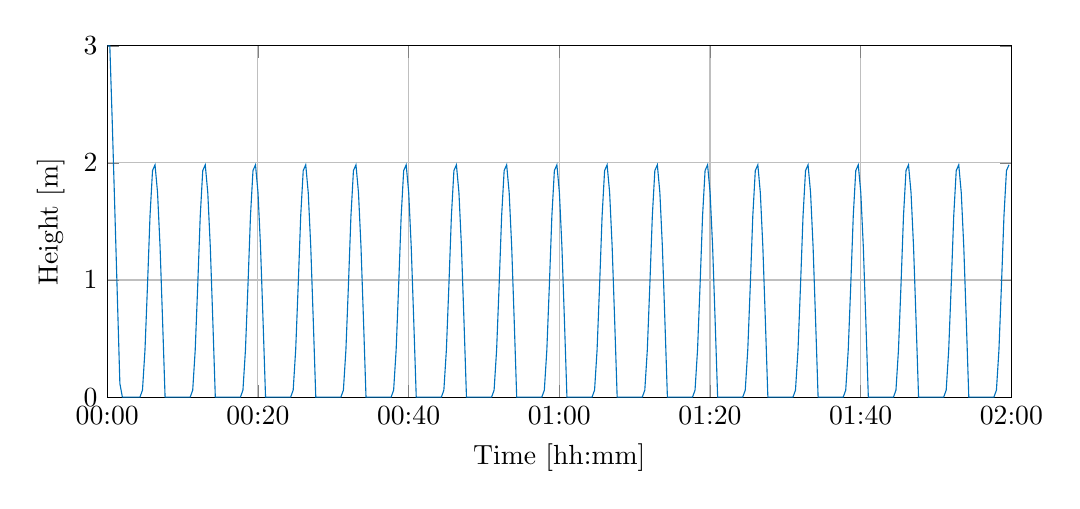
\begin{tikzpicture}

\begin{axis}[%
width=4.521in,
height=1.7566in,
at={(0.758in,0.481in)},
scale only axis,
xmin=0,
xmax=7200,
xtick={0,1200,2400,3600,4800,6000,7200},
xticklabels={{00:00},{00:20},{00:40},{01:00},{01:20},{01:40},{02:00},{},{}},
xlabel={Time [hh:mm]},
xmajorgrids,
ymin=0,
ymax=3,
ylabel={Height [m]},
ymajorgrids,
axis background/.style={fill=white}
]
\addplot [color=mycolor1,solid,forget plot]
  table[row sep=crcr]{%
1	3\\
21	2.99999999316026\\
41	2.32754415169987\\
61	1.59384668206183\\
81	0.855486505639804\\
101	0.11665418915018\\
121	0\\
141	0\\
161	0\\
181	0\\
201	0\\
221	0\\
241	0\\
261	0\\
281	0.0595953504678914\\
301	0.40302542412948\\
321	0.953696376221655\\
341	1.54661857226603\\
361	1.93450659540532\\
381	1.98368241475169\\
401	1.74649216864076\\
421	1.28645074216793\\
441	0.6571917603094\\
461	0\\
481	0\\
501	0\\
521	0\\
541	0\\
561	0\\
581	0\\
601	0\\
621	0\\
641	0\\
661	0\\
681	0.0595953504680377\\
701	0.403025424129614\\
721	0.953696376221789\\
741	1.54661857226616\\
761	1.93450659540545\\
781	1.98368241475182\\
801	1.74649216864089\\
821	1.28645074216806\\
841	0.657191760309528\\
861	0\\
881	0\\
901	0\\
921	0\\
941	0\\
961	0\\
981	0\\
1001	0\\
1021	0\\
1041	0\\
1061	0\\
1081	0.0595953504680377\\
1101	0.403025424129614\\
1121	0.953696376221789\\
1141	1.54661857226616\\
1161	1.93450659540545\\
1181	1.98368241475182\\
1201	1.74649216864089\\
1221	1.28645074216806\\
1241	0.657191760309528\\
1261	0\\
1281	0\\
1301	0\\
1321	0\\
1341	0\\
1361	0\\
1381	0\\
1401	0\\
1421	0\\
1441	0\\
1461	0\\
1481	0.0595953504680377\\
1501	0.403025424129614\\
1521	0.953696376221789\\
1541	1.54661857226616\\
1561	1.93450659540545\\
1581	1.98368241475182\\
1601	1.74649216864089\\
1621	1.28645074216806\\
1641	0.657191760309528\\
1661	0\\
1681	0\\
1701	0\\
1721	0\\
1741	0\\
1761	0\\
1781	0\\
1801	0\\
1821	0\\
1841	0\\
1861	0\\
1881	0.0595953504680377\\
1901	0.403025424129614\\
1921	0.953696376221789\\
1941	1.54661857226616\\
1961	1.93450659540545\\
1981	1.98368241475182\\
2001	1.74649216864089\\
2021	1.28645074216806\\
2041	0.657191760309528\\
2061	0\\
2081	0\\
2101	0\\
2121	0\\
2141	0\\
2161	0\\
2181	0\\
2201	0\\
2221	0\\
2241	0\\
2261	0\\
2281	0.0595953504680377\\
2301	0.403025424129614\\
2321	0.953696376221789\\
2341	1.54661857226616\\
2361	1.93450659540545\\
2381	1.98368241475182\\
2401	1.74649216864089\\
2421	1.28645074216806\\
2441	0.657191760309528\\
2461	0\\
2481	0\\
2501	0\\
2521	0\\
2541	0\\
2561	0\\
2581	0\\
2601	0\\
2621	0\\
2641	0\\
2661	0\\
2681	0.0595953504680377\\
2701	0.403025424129614\\
2721	0.953696376221789\\
2741	1.54661857226616\\
2761	1.93450659540545\\
2781	1.98368241475182\\
2801	1.74649216864089\\
2821	1.28645074216806\\
2841	0.657191760309528\\
2861	0\\
2881	0\\
2901	0\\
2921	0\\
2941	0\\
2961	0\\
2981	0\\
3001	0\\
3021	0\\
3041	0\\
3061	0\\
3081	0.0595953504680377\\
3101	0.403025424129614\\
3121	0.953696376221789\\
3141	1.54661857226616\\
3161	1.93450659540545\\
3181	1.98368241475182\\
3201	1.74649216864089\\
3221	1.28645074216806\\
3241	0.657191760309528\\
3261	0\\
3281	0\\
3301	0\\
3321	0\\
3341	0\\
3361	0\\
3381	0\\
3401	0\\
3421	0\\
3441	0\\
3461	0\\
3481	0.0595953504680377\\
3501	0.403025424129614\\
3521	0.953696376221789\\
3541	1.54661857226616\\
3561	1.93450659540545\\
3581	1.98368241475182\\
3601	1.74649216864089\\
3621	1.28645074216806\\
3641	0.657191760309528\\
3661	0\\
3681	0\\
3701	0\\
3721	0\\
3741	0\\
3761	0\\
3781	0\\
3801	0\\
3821	0\\
3841	0\\
3861	0\\
3881	0.0595953504680377\\
3901	0.403025424129614\\
3921	0.953696376221789\\
3941	1.54661857226616\\
3961	1.93450659540545\\
3981	1.98368241475182\\
4001	1.74649216864089\\
4021	1.28645074216806\\
4041	0.657191760309528\\
4061	0\\
4081	0\\
4101	0\\
4121	0\\
4141	0\\
4161	0\\
4181	0\\
4201	0\\
4221	0\\
4241	0\\
4261	0\\
4281	0.0595953504680377\\
4301	0.403025424129614\\
4321	0.953696376221789\\
4341	1.54661857226616\\
4361	1.93450659540545\\
4381	1.98368241475182\\
4401	1.74649216864089\\
4421	1.28645074216806\\
4441	0.657191760309528\\
4461	0\\
4481	0\\
4501	0\\
4521	0\\
4541	0\\
4561	0\\
4581	0\\
4601	0\\
4621	0\\
4641	0\\
4661	0\\
4681	0.0595953504680377\\
4701	0.403025424129614\\
4721	0.953696376221789\\
4741	1.54661857226616\\
4761	1.93450659540545\\
4781	1.98368241475182\\
4801	1.74649216864089\\
4821	1.28645074216806\\
4841	0.657191760309528\\
4861	0\\
4881	0\\
4901	0\\
4921	0\\
4941	0\\
4961	0\\
4981	0\\
5001	0\\
5021	0\\
5041	0\\
5061	0\\
5081	0.0595953504680377\\
5101	0.403025424129614\\
5121	0.953696376221789\\
5141	1.54661857226616\\
5161	1.93450659540545\\
5181	1.98368241475182\\
5201	1.74649216864089\\
5221	1.28645074216806\\
5241	0.657191760309528\\
5261	0\\
5281	0\\
5301	0\\
5321	0\\
5341	0\\
5361	0\\
5381	0\\
5401	0\\
5421	0\\
5441	0\\
5461	0\\
5481	0.0595953504680377\\
5501	0.403025424129614\\
5521	0.953696376221789\\
5541	1.54661857226616\\
5561	1.93450659540545\\
5581	1.98368241475182\\
5601	1.74649216864089\\
5621	1.28645074216806\\
5641	0.657191760309528\\
5661	0\\
5681	0\\
5701	0\\
5721	0\\
5741	0\\
5761	0\\
5781	0\\
5801	0\\
5821	0\\
5841	0\\
5861	0\\
5881	0.0595953504680377\\
5901	0.403025424129614\\
5921	0.953696376221789\\
5941	1.54661857226616\\
5961	1.93450659540545\\
5981	1.98368241475182\\
6001	1.74649216864089\\
6021	1.28645074216806\\
6041	0.657191760309528\\
6061	0\\
6081	0\\
6101	0\\
6121	0\\
6141	0\\
6161	0\\
6181	0\\
6201	0\\
6221	0\\
6241	0\\
6261	0\\
6281	0.0595953504680377\\
6301	0.403025424129614\\
6321	0.953696376221789\\
6341	1.54661857226616\\
6361	1.93450659540545\\
6381	1.98368241475182\\
6401	1.74649216864089\\
6421	1.28645074216806\\
6441	0.657191760309528\\
6461	0\\
6481	0\\
6501	0\\
6521	0\\
6541	0\\
6561	0\\
6581	0\\
6601	0\\
6621	0\\
6641	0\\
6661	0\\
6681	0.0595953504680377\\
6701	0.403025424129614\\
6721	0.953696376221789\\
6741	1.54661857226616\\
6761	1.93450659540545\\
6781	1.98368241475182\\
6801	1.74649216864089\\
6821	1.28645074216806\\
6841	0.657191760309528\\
6861	0\\
6881	0\\
6901	0\\
6921	0\\
6941	0\\
6961	0\\
6981	0\\
7001	0\\
7021	0\\
7041	0\\
7061	0\\
7081	0.0595953504680377\\
7101	0.403025424129614\\
7121	0.953696376221789\\
7141	1.54661857226616\\
7161	1.93450659540545\\
7181	1.98368241475182\\
};
\end{axis}
\end{tikzpicture}%
\caption{The height in the tank for the second simulation.}
\label{fig:tank_height_second_test_with_constraints}
\end{figure}

It can be seen that the tank does not get overfilled any more, thereby is within the constraints for the tank. At the beginning the tank is emptied again due to it was initials with wastewater in it. Hereafter the tank is filled to 2 meters and then emptied again. In figure \ref{fig:MPC_test_output_second_test_with_constraints} the output of the second pipe is shown. 

\begin{figure}[H]
 \centering
 % This file was created by matlab2tikz.
%
%The latest updates can be retrieved from
%  http://www.mathworks.com/matlabcentral/fileexchange/22022-matlab2tikz-matlab2tikz
%where you can also make suggestions and rate matlab2tikz.
%
\definecolor{mycolor1}{rgb}{0.00000,0.44700,0.74100}%
%
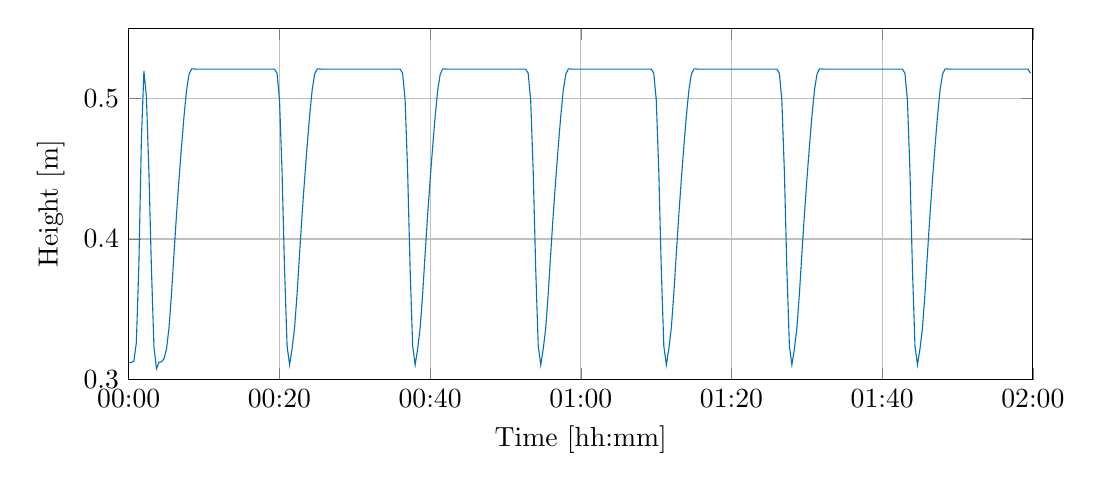
\begin{tikzpicture}

\begin{axis}[%
width=4.521in,
height=1.7566in,
at={(0.758in,0.481in)},
scale only axis,
xmin=0,
xmax=7200,
xtick={0,1200,2400,3600,4800,6000,7200},
xticklabels={{00:00},{00:20},{00:40},{01:00},{01:20},{01:40},{02:00},{},{}},
xlabel={Time [hh:mm]},
xmajorgrids,
ymin=0.3,
ymax=0.55,
ylabel={Height [m]},
ymajorgrids,
axis background/.style={fill=white}
]
\addplot [color=mycolor1,solid,forget plot]
  table[row sep=crcr]{%
1	0.312023251728134\\
21	0.312023249248491\\
41	0.313138414051669\\
61	0.326407936305141\\
81	0.381997703162978\\
101	0.470815867610163\\
121	0.519510061802365\\
141	0.501318732196232\\
161	0.446991990334918\\
181	0.378629775152903\\
201	0.323424080299287\\
221	0.307582010665573\\
241	0.312345479659611\\
261	0.312613834369712\\
281	0.314838075907383\\
301	0.321692488588001\\
321	0.336982577239558\\
341	0.361437149377047\\
361	0.390265428810376\\
381	0.417934720983639\\
401	0.443012153026768\\
421	0.466338666478772\\
441	0.48800305532753\\
461	0.506146824817801\\
481	0.517441377231075\\
501	0.521096113212522\\
521	0.521001898298191\\
541	0.520843966505831\\
561	0.520923224541938\\
581	0.520898876416836\\
601	0.520904713243865\\
621	0.520903514676294\\
641	0.520903736160123\\
661	0.520903698272369\\
681	0.520903704451414\\
701	0.520903703439729\\
721	0.520903703556692\\
741	0.520903703544504\\
761	0.520903703545671\\
781	0.520903703545567\\
801	0.520903703545576\\
821	0.520903703545574\\
841	0.520903703545575\\
861	0.520903703545575\\
881	0.520903703545574\\
901	0.520903703545575\\
921	0.520903703545575\\
941	0.520903703545574\\
961	0.520903703545575\\
981	0.520903703545575\\
1001	0.520903703545574\\
1021	0.520903703545575\\
1041	0.520903703545575\\
1061	0.520903703545574\\
1081	0.520903703545575\\
1101	0.520903703545575\\
1121	0.520903703545574\\
1141	0.520903703545575\\
1161	0.520903703545575\\
1181	0.518024144123985\\
1201	0.498769569060999\\
1221	0.448211924601428\\
1241	0.378364975971694\\
1261	0.32405196356739\\
1281	0.310412797128217\\
1301	0.321935680338255\\
1321	0.336970288985626\\
1341	0.361437845731993\\
1361	0.39026537866649\\
1381	0.417934725451377\\
1401	0.443012152566466\\
1421	0.466338666530941\\
1441	0.488003055321209\\
1461	0.506146824818603\\
1481	0.517441377230969\\
1501	0.521096113212535\\
1521	0.521001898298188\\
1541	0.52084396650583\\
1561	0.520923224541938\\
1581	0.520898876416836\\
1601	0.520904713243865\\
1621	0.520903514676294\\
1641	0.520903736160123\\
1661	0.520903698272369\\
1681	0.520903704451414\\
1701	0.520903703439729\\
1721	0.520903703556692\\
1741	0.520903703544504\\
1761	0.520903703545671\\
1781	0.520903703545567\\
1801	0.520903703545576\\
1821	0.520903703545574\\
1841	0.520903703545575\\
1861	0.520903703545575\\
1881	0.520903703545574\\
1901	0.520903703545575\\
1921	0.520903703545575\\
1941	0.520903703545574\\
1961	0.520903703545575\\
1981	0.520903703545575\\
2001	0.520903703545574\\
2021	0.520903703545575\\
2041	0.520903703545575\\
2061	0.520903703545574\\
2081	0.520903703545575\\
2101	0.520903703545575\\
2121	0.520903703545574\\
2141	0.520903703545575\\
2161	0.520903703545575\\
2181	0.518024144123985\\
2201	0.498769569060999\\
2221	0.448211924601428\\
2241	0.378364975971694\\
2261	0.32405196356739\\
2281	0.310412797128217\\
2301	0.321935680338255\\
2321	0.336970288985626\\
2341	0.361437845731993\\
2361	0.39026537866649\\
2381	0.417934725451377\\
2401	0.443012152566466\\
2421	0.466338666530941\\
2441	0.488003055321209\\
2461	0.506146824818603\\
2481	0.517441377230969\\
2501	0.521096113212535\\
2521	0.521001898298188\\
2541	0.52084396650583\\
2561	0.520923224541938\\
2581	0.520898876416836\\
2601	0.520904713243865\\
2621	0.520903514676294\\
2641	0.520903736160123\\
2661	0.520903698272369\\
2681	0.520903704451414\\
2701	0.520903703439729\\
2721	0.520903703556692\\
2741	0.520903703544504\\
2761	0.520903703545671\\
2781	0.520903703545567\\
2801	0.520903703545576\\
2821	0.520903703545574\\
2841	0.520903703545575\\
2861	0.520903703545575\\
2881	0.520903703545574\\
2901	0.520903703545575\\
2921	0.520903703545575\\
2941	0.520903703545574\\
2961	0.520903703545575\\
2981	0.520903703545575\\
3001	0.520903703545574\\
3021	0.520903703545575\\
3041	0.520903703545575\\
3061	0.520903703545574\\
3081	0.520903703545575\\
3101	0.520903703545575\\
3121	0.520903703545574\\
3141	0.520903703545575\\
3161	0.520903703545575\\
3181	0.518024144123985\\
3201	0.498769569060999\\
3221	0.448211924601428\\
3241	0.378364975971694\\
3261	0.32405196356739\\
3281	0.310412797128217\\
3301	0.321935680338255\\
3321	0.336970288985626\\
3341	0.361437845731993\\
3361	0.39026537866649\\
3381	0.417934725451377\\
3401	0.443012152566466\\
3421	0.466338666530941\\
3441	0.488003055321209\\
3461	0.506146824818603\\
3481	0.517441377230969\\
3501	0.521096113212535\\
3521	0.521001898298188\\
3541	0.52084396650583\\
3561	0.520923224541938\\
3581	0.520898876416836\\
3601	0.520904713243865\\
3621	0.520903514676294\\
3641	0.520903736160123\\
3661	0.520903698272369\\
3681	0.520903704451414\\
3701	0.520903703439729\\
3721	0.520903703556692\\
3741	0.520903703544504\\
3761	0.520903703545671\\
3781	0.520903703545567\\
3801	0.520903703545576\\
3821	0.520903703545574\\
3841	0.520903703545575\\
3861	0.520903703545575\\
3881	0.520903703545574\\
3901	0.520903703545575\\
3921	0.520903703545575\\
3941	0.520903703545574\\
3961	0.520903703545575\\
3981	0.520903703545575\\
4001	0.520903703545574\\
4021	0.520903703545575\\
4041	0.520903703545575\\
4061	0.520903703545574\\
4081	0.520903703545575\\
4101	0.520903703545575\\
4121	0.520903703545574\\
4141	0.520903703545575\\
4161	0.520903703545575\\
4181	0.518024144123985\\
4201	0.498769569060999\\
4221	0.448211924601428\\
4241	0.378364975971694\\
4261	0.32405196356739\\
4281	0.310412797128217\\
4301	0.321935680338255\\
4321	0.336970288985626\\
4341	0.361437845731993\\
4361	0.39026537866649\\
4381	0.417934725451377\\
4401	0.443012152566466\\
4421	0.466338666530941\\
4441	0.488003055321209\\
4461	0.506146824818603\\
4481	0.517441377230969\\
4501	0.521096113212535\\
4521	0.521001898298188\\
4541	0.52084396650583\\
4561	0.520923224541938\\
4581	0.520898876416836\\
4601	0.520904713243865\\
4621	0.520903514676294\\
4641	0.520903736160123\\
4661	0.520903698272369\\
4681	0.520903704451414\\
4701	0.520903703439729\\
4721	0.520903703556692\\
4741	0.520903703544504\\
4761	0.520903703545671\\
4781	0.520903703545567\\
4801	0.520903703545576\\
4821	0.520903703545574\\
4841	0.520903703545575\\
4861	0.520903703545575\\
4881	0.520903703545574\\
4901	0.520903703545575\\
4921	0.520903703545575\\
4941	0.520903703545574\\
4961	0.520903703545575\\
4981	0.520903703545575\\
5001	0.520903703545574\\
5021	0.520903703545575\\
5041	0.520903703545575\\
5061	0.520903703545574\\
5081	0.520903703545575\\
5101	0.520903703545575\\
5121	0.520903703545574\\
5141	0.520903703545575\\
5161	0.520903703545575\\
5181	0.518024144123985\\
5201	0.498769569060999\\
5221	0.448211924601428\\
5241	0.378364975971694\\
5261	0.32405196356739\\
5281	0.310412797128217\\
5301	0.321935680338255\\
5321	0.336970288985626\\
5341	0.361437845731993\\
5361	0.39026537866649\\
5381	0.417934725451377\\
5401	0.443012152566466\\
5421	0.466338666530941\\
5441	0.488003055321209\\
5461	0.506146824818603\\
5481	0.517441377230969\\
5501	0.521096113212535\\
5521	0.521001898298188\\
5541	0.52084396650583\\
5561	0.520923224541938\\
5581	0.520898876416836\\
5601	0.520904713243865\\
5621	0.520903514676294\\
5641	0.520903736160123\\
5661	0.520903698272369\\
5681	0.520903704451414\\
5701	0.520903703439729\\
5721	0.520903703556692\\
5741	0.520903703544504\\
5761	0.520903703545671\\
5781	0.520903703545567\\
5801	0.520903703545576\\
5821	0.520903703545574\\
5841	0.520903703545575\\
5861	0.520903703545575\\
5881	0.520903703545574\\
5901	0.520903703545575\\
5921	0.520903703545575\\
5941	0.520903703545574\\
5961	0.520903703545575\\
5981	0.520903703545575\\
6001	0.520903703545574\\
6021	0.520903703545575\\
6041	0.520903703545575\\
6061	0.520903703545574\\
6081	0.520903703545575\\
6101	0.520903703545575\\
6121	0.520903703545574\\
6141	0.520903703545575\\
6161	0.520903703545575\\
6181	0.518024144123985\\
6201	0.498769569060999\\
6221	0.448211924601428\\
6241	0.378364975971694\\
6261	0.32405196356739\\
6281	0.310412797128217\\
6301	0.321935680338255\\
6321	0.336970288985626\\
6341	0.361437845731993\\
6361	0.39026537866649\\
6381	0.417934725451377\\
6401	0.443012152566466\\
6421	0.466338666530941\\
6441	0.488003055321209\\
6461	0.506146824818603\\
6481	0.517441377230969\\
6501	0.521096113212535\\
6521	0.521001898298188\\
6541	0.52084396650583\\
6561	0.520923224541938\\
6581	0.520898876416836\\
6601	0.520904713243865\\
6621	0.520903514676294\\
6641	0.520903736160123\\
6661	0.520903698272369\\
6681	0.520903704451414\\
6701	0.520903703439729\\
6721	0.520903703556692\\
6741	0.520903703544504\\
6761	0.520903703545671\\
6781	0.520903703545567\\
6801	0.520903703545576\\
6821	0.520903703545574\\
6841	0.520903703545575\\
6861	0.520903703545575\\
6881	0.520903703545574\\
6901	0.520903703545575\\
6921	0.520903703545575\\
6941	0.520903703545574\\
6961	0.520903703545575\\
6981	0.520903703545575\\
7001	0.520903703545574\\
7021	0.520903703545575\\
7041	0.520903703545575\\
7061	0.520903703545574\\
7081	0.520903703545575\\
7101	0.520903703545575\\
7121	0.520903703545574\\
7141	0.520903703545575\\
7161	0.520903703545575\\
7181	0.518024144123985\\
};
\end{axis}
\end{tikzpicture}%
\caption{The output of the last pipe.}
\label{fig:MPC_test_output_second_test_with_constraints}
\end{figure}

It is clear from the figure that the output is not even close to be constant. I fluctuates between two values, the constant input, approximately 0,31 meters, and 0,51 meters. In the top and bottom of the curve, it can be seen that the curve level off. The bottom is due to the tank is empty and therefore, the input, that goes into the tank from the first pipe, goes right into the second pipe without storing any wastewater in the tank. When the top levels off the tank starts to be filled up and as it goes down the tank is emptied. It was discovered that the reason for the top is due to constraints on the upper bound for the input, this however is not a wanted feature. It was desired to get a constant output or a minimum of variations in the output, which is not achieved. Through several tries of changing the parameters of the constraints, e.g. lessen the controller constraint a solution was not found, in every case the output looked similar to the one shown in figure \ref{fig:MPC_test_output_second_test_with_constraints}.

           





